\chapter{Implementation}\label{ch:implementation}

In this chapter we will explain how the system was implemented, so we will describe 
technologies/languages, data structures, patterns and best practices used.


\section{Tools}


\subsection{Language}


The best choice between the languages exposed during the course seems to be 
\textbf{Erlang}~\cite{3}; 
in fact \textbf{Erlang OTP} allows to handle concurrency and distributed programming
moreover provides some \textbf{behaviours} really useful for this project:
\begin{itemize}
    \item \textbf{gen$\_$statem behaviour} allows to create a \textbf{finite state machine} 
        based on events (that fits perfectly with the nature of the problem);
    \item \textbf{gen$\_$server behaviour} allows to create a \textbf{web server}; 
        anyway for the web service implementation we prefer to use a more 
        rich and well documented \textbf{web framework} called \textbf{Cowboy}~\cite{4}  
\end{itemize}


\subsection{Web service}

Thanks to Cowboy we were able to implement a web service that exposes a \textbf{RESTful API}  
for both cars and simulation clients; we use \textbf{JSON}~\cite{6} as standard data interchange 
format for any interaction with the web service APIs.

The main reason of this decision is that it is, nowadays, a standard de facto and also 
versatile/\textbf{independent from the language} used 
(we use a library called \textbf{Jiffy}~\cite{5} for serialization/deserialization of data).


\subsubsection{Patterns and best practices}

The web service architecture follows the idea on the base of the \textbf{MVC pattern}; 
views, models and controllers were splitted and located in different files. 

The \textbf{front-end tier} is structured in views, stored in the same folder of the 
back-end code (for scope reasons). 
Each view can calls the server calling \textit{http-client.js} 
functions that use \textbf{AJAX}~\cite{12} for HTTP calls. 

The \textbf{back-end tier} follows also the \textbf{repository pattern} and 
\textbf{CRUD}~\cite{13} logic 
for what concerns the interaction with Mnesia. We decide to use the repository pattern 
in order to feel free, at any time, to change DBMS/connect with more than one DB without 
rewrite business logic code.

Mnesia is a no-SQL DBMS that basically works in a functional way (it is written in Erlang)
with tuples so it \textbf{isn't necessary any kind of ORM}~\cite{7} in order 
to map query results with Erlang data structures (and also avoid some issues of SQL 
like \lq\lq hard-coded\rq\rq\ queries and SQL-injection~\cite{8}).

Moreover every query, in particular \textbf{commands} (non idempotent query defined in 
CQRS~\cite{14} pattern), is made with a \textbf{transaction} so concurrency 
doesn't constitue an issue for this architecture.\\

\noindent
An HTTP call flow is really simple and clear; it starts from the \textbf{routing module} 
\textit{web$\_$service$\_$app.erl} that forwards the request to the right 
\textbf{controller}. In this passage we can also interpone some \textbf{middlewares} 
but the project doesn't require any.

\textbf{Controllers} are responsible for data unmarshalling and 
call \textbf{business logic routines}. 

The entire logic of the web service is 
stored into the \textbf{service layer} that has the duty to interact with 
the database using the interfaces exponed by the repositories and returns to 
the controller the expected results. For this reason in order to \textbf{test} 
the business logic is enough to test the utility functions used and exponed 
by the services.  

The module dependencies are: \textit{cowboy}, \textit{jiffy} and \textit{rebar3$\_$run} 
plugin; \textbf{dependency management} was delegated to \textbf{rebar3}~\cite{17} 
that uses internally HEX~\cite{18} package manger.


\subsection{UI}

UI is implemented using some famous front-end libraries collected with 
\textbf{npm}~\cite{16} package manager. 

Client UI can be used in any context so must have a \textbf{responsive layout} in order 
to fit any screen size; we use \textbf{Bootstrap}~\cite{19} and JQuery~\cite{20} 
in order to create a fluid layout. 

Moreover we though that the aesthetics of the simulation could be more appealing 
using \textbf{ThreeJS}~\cite{21} so we have injected in the main view a \textbf{3D canvas} 
where cars are rendered as blocks on a 2D street plane.


\subsection{Car}

Car is structured as a \textbf{finite state machine} with events, 
it has a \textbf{supervisor} that initializes the FSM and manages the interactions 
with the other cars and with the web service. 

The initial idea was to exclude the supervisor and call another car directly sending 
a message; this idea fails cause $gen\_statem$ behaviour doesn't allow to send/receive 
messages such as a normal node. 

So the behavior forces to \textbf{use the supervisor as an interface} with the FSM 
moreover we want to realize an asynchronous system for message exchange also 
capable to keep track of message RTT and other parameters. 

The solution was the creation of a little \textbf{timer subprocess} that manages the 
message exchange; this way was applicable but also a little complex because 
a message between two cars requires 8 hops (4 hops for the request and 4 hops for 
the response) so we implement a \textbf{pseudo multi-layer encapsulation} in order 
to create a generic asynchronous communication infrastructure.    

\begin{center}
    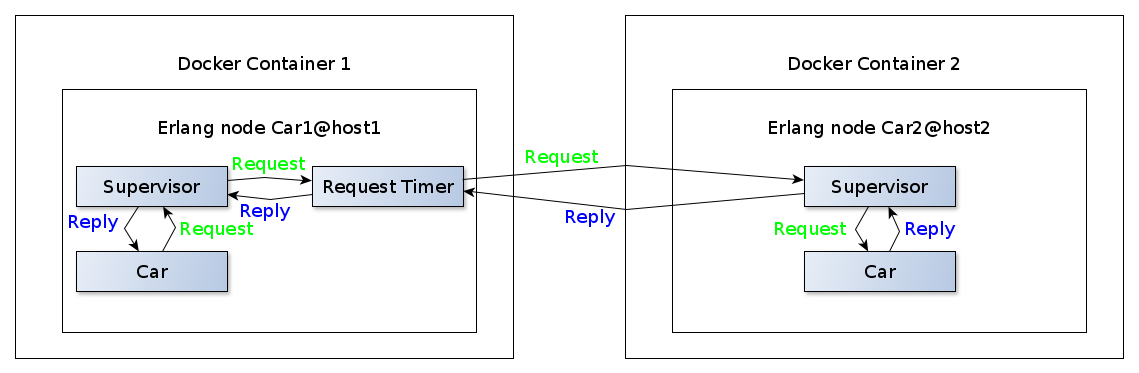
\includegraphics[scale=0.3]{assets/request-track.png}
    \captionof{figure}{Message exchange between two cars}
\end{center}
\begin{center}
    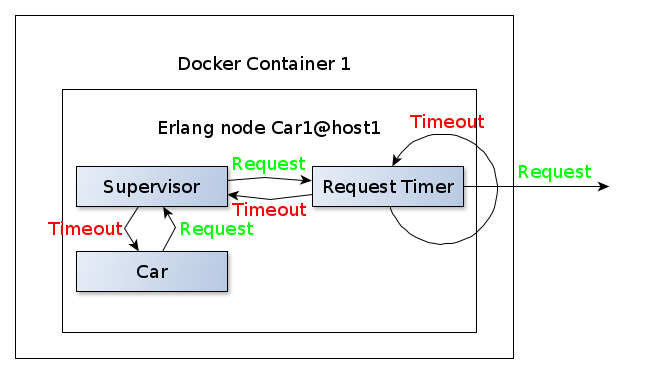
\includegraphics[scale=0.3]{assets/request-timeout.png}
    \captionof{figure}{A message without any reply triggers a timeout event}
\end{center}


\section{Docker}

At the end of the implementation the Erlang scripts were builded inside a docker image 
ready to be instantiated in a new container. 

Cars aren't aware, at compile time, of the \textbf{parameters} that characterize them 
(size, power, global settings, web server IP, etc.) so we exploit 
the docker feature to pass arguments with the \textit{run} call in order to 
\textbf{initialize the car}.  

Now the web service is sandboxed in a Docker container so in order to be able to launch 
bash commands (ie. to raise a new car instance) outside its scope we set up an 
\textbf{SSH tunnel}~\cite{15} toward the target host.


\section{Data structures}

As described in Chaper 1, cars and bridge must be aware about their characteristics.

In order to do that we have decided to create an environment file 
(\textit{environment.json}) that collects the default environment settings,
flanked by the UI that allows to update some settings.   


\subsection{Environment}
------TODO

To model the environment the following attributes, which are set in environment.js for once, will be used:
\begin{itemize}
    \item $host$:\\ Web service IP:PORT
    \item $max\_speed$:\\ the maximun speed allowed
    \item $bridge\_capacity$: number\\ it defines the maximun number of cars that can cross the bridge
    at the same time
    \item $bridge\_length$: number\\ it defines the lenght of the bridge
    \item $tow\_truck\_time$: number\\ time necessary for the tow truck to arrive and remove the dead car
    \item $max\_RTT$:number\\ it is the maximun RTT that could happen
\end{itemize}

These attributes will never be modified during the simulation.

\subsection{Car}
------TODO
Each car A is modelled exploiting the following attributes:
\begin{itemize}
    \item $name$: integer\\ it identifies univocally the car
    \item $side$: {1, -1}\\ if equal to 1 means that the car is on the right side, 
    if equal to -1 it means that it is on left side
    \item $power$: integer\\ it defines the number of rear and front cars that the car can reach
    \item $size$: integer \\ it defines the lenght of the car
    \item $speed$: number\\ it defines the distance that the car goes through in one turn\\
    it has a maximun value specified in \textbf{environment.js}\\
    it is initialized with 0 to prevent crashing 
    \item $crossing$: boolean\\ if true it means that the car is on the bridge
    \item $syncrhonized$: boolean\\ if true it means that the car is syncrhonized    
    \item $crash_type$: {0, 1, 2}\\ if equal to zero, the car won't crash, if equal to one the car will have an engine only crash
    and if equal to 2 the car will have both engine and system crash 
    \item $delta$: number\\ it is the difference between the local time and the global time
    \item $adj$: another data structure\\ it contains the lists of front and rear cars
    \item $state$: string\\ it defines the current state of the car\\ it could be \textbf{init}, \textbf{sync}, \textbf{normal} or \textbf{dead}
    \item $position$: number \\it indicates the distance between the car and the bridge or the car and the end of the
    bridge\\it is initialized as $pos(B)+1*side(B)$, where B is the first front car, if B is on the same side of A, or
    as $-pos(B)$ if B is on the other side\\ when negative it means that the car is on the left side, otherwise on the right side
    \item $arrival\_time$: number\\ it defines the time when the car has arrived in the queue
    \item $current\_time$: number\\ it indicates the local time at each turn
\end{itemize}
These above are the car metadata, while the following are settings and bridge metadata 
(these are taken from the environment definition but must be part of the car specifics too):
\begin{itemize}
    \item $host$:\\ Web service IP
    \item $bridge\_capacity$: number\\ it defines the maximun number of cars that can cross the bridge
    at the same time
    \item $bridge\_length$: number\\ it defines the lenght of the bridge
    \item $max\_speed$:\\ the maximun speed allowed
    \item $tow\_truck\_time$: number\\ time necessary for the tow truck to arrive and remove the dead car
    \item $max\_RTT$:number\\ it is the maximun RTT that could happen
    \item $port$:\\ Web service PORT
\end{itemize}

Note that $bridge\_capacity$ and $bridge\_length$ are imposed by the environment and cannot change during the
simulation. Furthermore $name$ and $power$ are defined independently, while $delta$ and $adj$ 
depend on the other cars.\\

We choose to model the car as a finite state machine because the car can switch between four main different states. 
\subsection{Init}

Init isn't properly a state cause cannot receive external events, 
is used only for 
\textit{Data}\footnote{\textbf{Data}: we denote as \textit{Data} 
the state persistent variables} 
initializations.


\subsection{Sync}

After FSM initialization the car reaches \textbf{sync state}, the main goals 
of this state are:

\begin{itemize}
    \item Synchronize with the other cars
    \item Set a consistent arrival time with the queue state 
    \item Set an initial position (safe, avoid spawn on the other cars)
    \item Send an update to the DB layer with the informations above
\end{itemize}

In order to perform a synchronization using Berkeley algorithm the new car needs to 
know a reference of the last car in the queue which is exposed by an end point; 
in order to avoid concurrency issues when a car calls the end point 
it becomes automatically the last car in the queue (with a transaction query).

This implies that any car is chained with the car in front of her and any other 
new car, from now on, cannot be interponed betweent them.\\

\noindent
If everything goes in the right way, at the end of the synchronization the new car ($A$) 
is located near the car in front of her ($B$) and the arrival time of $A$ must be 
higher then that of $B$.

We have also to guarantee \textbf{I} property so a car in sync state can synchronize 
itself with the database layer only after the car in front of her. Define 
$A:check(B)$ a check message from $A$ to $B$ that asks for the current $B$ state;
the message reply contains every relevant information about $B$ also its synchronization 
state, so is enough to wait until a check response state that B was just 
synchronized.  

If a check call doesn't have any reply, a timeout event will be triggered after 
$max_{RTT}$ ms. Once a car receives a timeout event calls a special process 
tow truck that has the duty of remove the broken cars.  

Once a car is removed by a tow truck the garbage process returns to the caller 
an update event that is then propagated to every other cars. For this kind of events 
the order isn't relevant, so even if we receive two concurrent updates of near cars 
we haven't to straggle to ordering them.


\subsection{Normal}

Sync was a static state, the car declares its initial position but has $speed_A = 0$;
normal is instead the state in which the car remains for the most of its life time and 
manages every car movement.

Assume that between two cars $A \rightarrow B$, in a certain instant $t_0$, 
there is a safety distance $d_{AB0}$; 
the car behind know this information because has sended a check message to the car 
in front of her and at instant $t_1$ receives a response.

Now $A$ is free to move forward (because $B$ can only move forward) of:

\begin{equation}\begin{split}
    & min\{\ d_{AB0},\ max\_speed * travel\_time \} \\
    & p_{Bi} \leq p_{Bj},\quad i < j \\
\end{split}\end{equation}    

Where $max\_speed$ is an arbitrary constant that constitute an upper bound for the speed 
and $travel\_time$ the time passed from the last car transition. 

Such as for sync also in this context we have to guarantee \textbf{I} property, so 
a car behind can move only after the car in front is synchronized with the DB layer.

Once a car reaches the bridge side and the car on the other side has an 
higher arrival time, the first car becomes the new leader.


\subsection{Leader}

Leader state is a static state such as sync, in this state the car notifies to 
the first $i$ rear cars the arrival time of of the car on the opposite side of the bridge 
(where $i$ is the bridge capacity) with a crossing message.

After the crossing propagation leader returns in the normal state in order to 
crossing the bridge. 

This simple leader election is safe, in the worst scenario 
the car in front can present a wrong arrival time due to a synchronization error 
but this at most cause the break of the FIFO order but never a car accident.


\subsection{Dead}

Once a car reaches the end of the bridge goes in the dead state and, 
after the sending of a global update event, the process stops.

A car can also reach dead from normal and leader states in case of an unexpected 
crash; in this case the car has to wait for a tow truck that removes it from the 
street. 

\subsubsection{Communication}

It is important to underline how two cars can send message to each other. \\
First of all, each car has a supervisor and, when a car A wants to send something to another car B,
this happens:
\begin{itemize}
   \item[1.] A sends a message to hers supervisor S$_{A}$
   \item [2.] S$_{A}$ calls a process, we can refer at it as $Timer$, which is used to send a timeout
   if the supervisor didn't receive a response from the other within a certain time. In that case S$_{A}$ assumes 
   that B is dead and so A will call a tow truck to remove it.
   \item[3.] S$_{A}$ sends it to the supervisor of B S$_{B}$
   \item [4.] S$_{B}$ sends an event to B which contains the message of A
   \item [5.] B sends a message to S$_{B}$ whit the response
   \item [6.] S$_{B}$ sends it to S$_{A}$, going through the $Timer$ as S$_{A}$ has done at point 2
   \item [7.] finally S$_{A}$ sends another event to A with the response of B, to which A reacts appropiately
\end{itemize}

\subsection{Adj}
We used another data structure for the adiacents cars, called $adj$:
\begin{itemize}
    \item $front\_cars$: list of cars\\ it contains all the car ahead that are rechable\\ the first element
     is the next car
    \item $rear\_cars$: list of cars\\ it contains all the car behind that are rechable\\ the last element
     is the previous car
\end{itemize} 